 
% Copyright 2004 by Till Tantau <tantau@users.sourceforge.net>.
%
% In principle, this file can be redistributed and/or modified under
% the terms of the GNU Public License, version 2.
%
% However, this file is supposed to be a template to be modified
% for your own needs. For this reason, if you use this file as a
% template and not specifically distribute it as part of a another
% package/program, I grant the extra permission to freely copy and
% modify this file as you see fit and even to delete this copyright
% notice. 
\AtBeginDocument{\renewcommand{\bibname}{References}}

\documentclass{beamer}
%\usepackage[table]{xcolor}
\usepackage[absolute,overlay,showboxes]{textpos}
\usepackage{caption}
\usepackage{xcolor,colortbl}
\usepackage{amsmath}
%\usepackage{lipsum}
%\AtBeginDocument{\renewcommand{\bibname}{References}}

% There are many different themes available for Beamer. A comprehensive
% list with examples is given here:
% http://deic.uab.es/~iblanes/beamer_gallery/index_by_theme.html
% You can uncomment the themes below if you would like to use a different
% one:
%\usetheme{AnnArbor}
%\usetheme{Antibes}
%\usetheme{Bergen}
%\usetheme{Berkeley}
%\usetheme{Berlin}
%\usetheme{Boadilla}
%\usetheme{boxes}
%\usetheme{CambridgeUS}
%\usetheme{Copenhagen}
%\usetheme{Darmstadt}
\usetheme{default}
%\usetheme{Frankfurt}
%\usetheme{Goettingen}
%\usetheme{Hannover}
%\usetheme{Ilmenau}
%\usetheme{JuanLesPins}
%\usetheme{Luebeck}
%\usetheme{Madrid}
%\usetheme{Malmoe}
%\usetheme{Marburg}
%\usetheme{Montpellier}
%\usetheme{PaloAlto}
%\usetheme{Pittsburgh}
%\usetheme{Rochester}
%\usetheme{Singapore}
%\usetheme{Szeged}
%\usetheme{Warsaw}

\title{Uplink User-Assisted Relaying in Cellular Networks}

% A subtitle is optional and this may be deleted
%\subtitle{Dual Degree Phase 1 Presentation}

\author{Presented by: Prudhvi Porandla \\ \quad (110070039)\\
\vspace{2mm}
Guide: Prof. S. N. Merchant \\
\vspace{2mm}
Dual Degree Phase 1 Presentation}
% - Give the names in the same order as the appear in the paper.
% - Use the \inst{?} command only if the authors have different
%   affiliation.

% - Use the \inst command only if there are several affiliations.
% - Keep it simple, no one is interested in your street address.

\date{October 27, 2015}
% - Either use conference name or its abbreviation.
% - Not really informative to the audience, more for people (including
%   yourself) who are reading the slides online

%%%%%\subject{Theoretical Computer Science}
% This is only inserted into the PDF information catalog. Can be left
% out. 

% If you have a file called "university-logo-filename.xxx", where xxx
% is a graphic format that can be processed by latex or pdflatex,
% resp., then you can add a logo as follows:

% \pgfdeclareimage[height=0.5cm]{university-logo}{university-logo-filename}
% \logo{\pgfuseimage{university-logo}}

% Delete this, if you do not want the table of contents to pop up at
% the beginning of each subsection:


% Let's get started
\begin{document}

\begin{frame}
  \titlepage
\end{frame}

\begin{frame}{Overview}
  \begin{itemize}
  \item Introduction
  \vspace{3mm}
  \item  Partial Decode-and-Forward Relaying
  \vspace{3mm}
  \item PDF in Cellular Networks
  \vspace{3mm}
  \item Cooperation Policies 
  \vspace{3mm}
  \item Simulations and Results
  \vspace{3mm}
  \item Future Work
  \end{itemize}
  % You might wish to add the option [pausesections]
\end{frame}

% Section and subsections will appear in the presentation overview
% and table of contents.



\begin{frame}{Introduction}
  \begin{itemize}
  \item Relaying cooperative communications will play important roles in future generations wireless networks.
  \vspace{0.5cm}
  \item Relay-aided cooperative communication techniques represent a promising technology that improves average rate
  \vspace{0.5cm}
  \item We use Partial Decode-and-Forward scheme for relaying
  \vspace{0.5cm}
  \item We will explore two policies by which active User Equipments(UEs) pick their relays
  \end{itemize}
  % You might wish to add the option [pausesections]
\end{frame}
%%%%\section{Second Main Section}

\begin{frame}{Partial Decode-and-Forward Relaying} {Two Phases}
Total transmission period is divided into phases: 1. Broadcast phase and 2. Multicast phase as shown in the figure below.
\begin{figure}
\centering
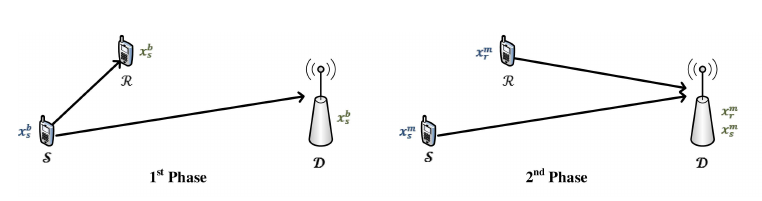
\includegraphics[width=\textwidth]{figures/pdfRelaying.png}
  \caption{Two phases in PDF relaying.}
\end{figure}
\end{frame}

\begin{frame}{Partial Decode-and-Forward Relaying} {Transmit Signals}
\vspace{-1cm}
The signals transmitted by source and relay are as follows:
\begin{align*}
\text{Phase 1:}\quad x^b_s &= \sqrt{P_s^b} U_s^b, \\
\text{Phase 2:}\quad x_r^m &= \sqrt{P_r^m}U_s^{m_1}, \\ 
 x^m_s &= \sqrt{P_s^{m_1}}U_s^{m_1} + \sqrt{P_s^{m_2}}V_s^{m_2} 
\end{align*}
\vspace{-0.5cm}
\begin{itemize}
\item All codewords above are picked from independent Gaussian codebooks with zero mean and unit variance.
\item $\alpha_1 P_s^b + \alpha_2 P_s^m = P_s, P_s^{m_1}+P_s^{m_2} = P_s^m,  \alpha_2P_r^m = P_r$
where $\alpha_2 = 1-\alpha_1$
\end{itemize}
\end{frame}

\begin{frame}{Partial Decode-and-Forward Relaying} {Received Signals}
\vspace{-1cm}
Signals received at relay, BS during broadcast(b) and multicast(m) phases:
\begin{equation*}
Y_r^b = h_{sr}x^b_s + Z_r^b , \quad Y_d^b = h_{sd}x^b_s + Z_d^b
\end{equation*}
$Z_r^b$ and $Z_d^b$ are \textit{i.i.d} $\mathcal{CN}(0,\sigma^2)$ that represent noises at $\mathcal{R}$ and $\mathcal{D}$. \\
\begin{equation*}
Y_d^m = h_{sd}x^m_s + h_{rd}x_r^m + Z_d^m
\end{equation*}
The above expression is true only if $\mathcal{D}$ has knowledge about the phase offset between $\mathcal{S}$ and $\mathcal{R}$. 
\end{frame}


\begin{frame}{Partial Decode-and-Forward Relaying} {Achievable Rate}
\vspace{-1cm}
With received signals as above and joint ML decoding rule at destination, the achievable rate for this relaying scheme is:
\begin{equation*} \label{eq:rate}
R_{PDF} \leq min(C_1+C_2,C_3)
\end{equation*}
\begin{align*}
\text{where } C_1 &= \alpha_1 \log\Big(1+|h_{sr}|^2P_s^b\Big),\\
C_2 &= \alpha_2 \log\Big(1+|h_{sd}|^2P_s^{m_2}\Big),\\
C_3 &= \alpha_1 \log\Big(1+|h_{sd}|^2P_s^b\Big) \\ &+ \alpha_2\log\bigg(1+|h_{sd}|^2P_s^{m_2} + \Big(|h_{sd}|\sqrt{P_s^{m_1}} + |h_{rd}|\sqrt{P_r^m}\Big)^2\bigg)
\end{align*}
\end{frame}

\begin{frame}{PDF in Cellular Networks}{Network Geometry}

\begin{itemize}
\item Active users in different cells using same resource block are are distributed according to a homogeneous and stationary Poisson point process (PPP) $\Phi_1$ with intensity $\lambda_1$
\item Idle UEs that can participate in relaying are distributed according to another PPP $\Phi_2$ with intensity $\lambda_2$.
\item $\Phi_1$ and $\Phi_2$ are independent.
\item BS is uniformly distributed in the Voronoi cell of its served UE
\end{itemize}
\end{frame}

\begin{frame}{PDF in Cellular Networks}{Network Geometry}
\begin{figure}
\centering
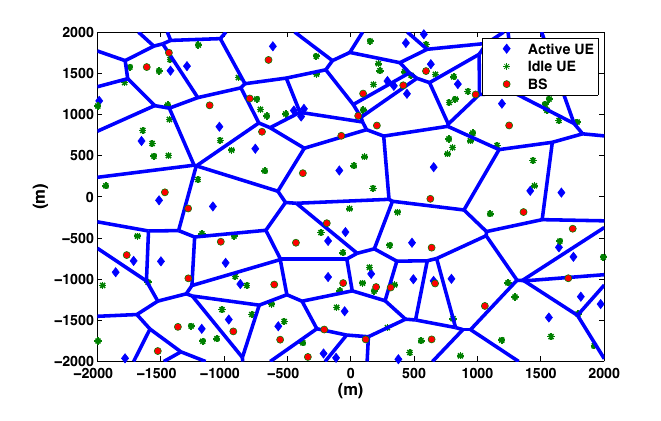
\includegraphics[width=\textwidth]{figures/netLayoutPaper.png}
  \caption{Sample Network Layout}
\end{figure}
\end{frame}

\begin{frame}{PDF in Cellular Networks}{Channel Model}

Consider $i^{th}$ active UE, we model the received signals at the relay and base station in this cell during 1st phase as
\begin{equation*}
Y_{r,i}^b = h^{(i)}_{sr}x_{s,i}^b + I_{r,i}^b + Z_{r,i}^b,
\end{equation*}
\begin{equation*}
Y_{d,i}^b = h^{(i)}_{sd}x_{s,i}^b + I_{d,i}^b + Z_{d,i}^b
\end{equation*}
where $I_{r,i}^b$ and $I_{d,i}^b$ represent the interference received at the $i^{th}$ relay and destination. 
In second phase of the transmission, the received signal at the BS can be modelled as 
\begin{equation*}
Y_{d,i}^m = h^{(i)}_{sd}x_{s,i}^m + h^{(i)}_{rd}x_{r,i}^m+ I_{d,i}^m + Z_{d,i}^m
\end{equation*}
\end{frame}

\begin{frame}{PDF in Cellular Networks}{Interference}
\begin{equation*} 
I_{r,i}^b = \sum_{k \neq i} B_k h^{(k,i)}_{sr} x_{s,k}^b + (1-B_k)h_{sr}^{(k,i)}x_{s,k} ,
\end{equation*}
\begin{equation*}
I_{d,i}^b = \sum_{k \neq i} B_k h_{sd}^{(k,i)} x^b_{s,k} + (1-B_k)h_{sd}^{(k,i)}x_{s,k},
\end{equation*}
\begin{equation*} \label{eq:interferences}
I_{d,i}^m = \sum_{k \neq i} B_k \Big(h_{sd}^{(k,i)} x^m_{s,k} + h_{rd}^{(k,i)} x^m_{r,k}\Big) + (1-B_k)h_{sd}^{(k,i)}x_{s,k}
\end{equation*}
where $B_k = 1$ if $k^{th}$ user has a relay. $B_k$ can be seen as a Bernoulli RV with success probability equal to cooperation probability of the policy by which relays are picked  
\end{frame}

\begin{frame}{PDF in Cellular Networks}{Interference}
\begin{itemize}
\item Interference at either the relay or destination is the
sum of many signals undergoing independent fading from nodes distributed in the infinite 2-D plane
\item Approximate the interference as a complex Gaussian distribution by using law of large numbers
\item Distributions: $ I_{d,i}^b \sim \mathcal{CN} (0,\mathcal{Q}_{d,i}^b), I_{d,i}
^m \sim \mathcal{CN}(0,\mathcal{Q}_{d,i}^m),$ and $I_{r,i}^b \sim \mathcal{CN}
(0,\mathcal{Q}_{r,i})$
\end{itemize}
\end{frame}

\begin{frame}{PDF in Cellular Networks}{Equivalent Standard Channel Model}
\begin{align*}
\tilde{Y}_{r,i}^b &= \tilde{h}_{sr}^{(i)}x_{s,i}^b + \tilde{Z}_{r,i}^b, \\
\tilde{Y}_{d,i}^b &= \tilde{h}_{sd}^{(i)}x_{s,i}^b + \tilde{Z}_{d,i}^b, \\
\tilde{Y}_{d,i}^m &= \tilde{h}_{sd}^{(i)}x_{s,i}^m + \tilde{h}_{rd}^{(i)}x_{r,i}^m + \tilde{Z}_{d,i}^m
\end{align*}
where the new channel fading terms are defined as

\begin{equation*}
\tilde{h}_{sr}^{(i)} = \frac{h_{sr}^{(i)}}{\sqrt{\mathcal{Q}_{r,i} + \sigma^2}}, \quad \tilde{h}_{sd}^{(b,i)} = \frac{h_{sd}^{(i)}}{\sqrt{\mathcal{Q}_{d,i}^b + \sigma^2}} 
\end{equation*}
\begin{equation*}
\tilde{h}_{sd}^{(m,i)} = \frac{h_{sd}^{(i)}}{\sqrt{\mathcal{Q}_{d,i}^m + \sigma^2}},
\quad \tilde{h}_{rd}^{(i)} = \frac{h_{rd}^{(i)}}{\sqrt{\mathcal{Q}_{d,i}^m + \sigma^2}}
\end{equation*}
and the noise terms are now all $\mathcal{CN}(0,1)$
\end{frame}




\begin{frame}{Cooperation Policies} {Ideal Policy $E_1$ }

\begin{align*}
E_1 &= \Big\{|\tilde{h}_{(sr)}^{(k)}|^2 \geq |\tilde{h}_{(sd)}^{(k)}|^2\Big\} \\
&\backsimeq \Big\{ \frac{g_{sr}r_2^{-\alpha}}{\mathcal{Q}_{r,k}} \geq \frac{g_{sd}r_1^{-\alpha}}{\mathcal{Q}_{d,k}^b} \Big\}
\end{align*}
where $r_1$ and $r_2$ denote the direct distance
between $\mathcal{S}$ and $\mathcal{D}$ and cooperation distance between $\mathcal{S}$ and its closest idle UE, respectively and $\alpha$ is pathloss exponent.
Active UE nodes should know instantaneous  SINRs of the relay link($\mathcal{S}-\mathcal{R}$) and the
direct link($\mathcal{S}-\mathcal{D}$)
\end{frame}

\begin{frame}{Cooperation Policies} {Pure Geometric Policy $E_2$}
\vspace{-1cm}
\begin{equation*}
E_2 = \{r_2\leq r_1, D \leq r_1 \}
\end{equation*}
where $D$ is the distance between $\mathcal{R}$ and $\mathcal{D}$.
\vspace{1cm}
\pause
\begin{itemize}
\item More practical than $E_1$ 
\pause
\item Does not require full knowledge of interference at decision making node. 
\pause
\item Only requires the decision making nodes to know the distances
from the active user to the nearest idle user and to the base
station. 
\end{itemize}
\end{frame}

\begin{frame}{Cooperation Policies} {Hybrid Policy $E_3$}
This policy is proposed for slow fading channels where small scale fading parameters estimation and their
feedback to the decision making node is feasible. 
\begin{equation*}
E_3 = \{g_{sd}r_1^{-\alpha} \leq g_{sr}r_2^{-\alpha}, D \leq r_1 \}
\end{equation*}
Note that this cooperation policy is still independent of the
interference as in the pure geometric cooperation policy $E_2$.
\end{frame}


\begin{frame}{Cooperation Probabilities} {Distributions of $r_1$,$r_2$}
The distribution of the distance
$r_1$ between the $i^{th}$ UE and its associated BS can be shown to
be Rayleigh distributed 
\begin{equation*}
f_{r_1}(r_1) = 2\pi\lambda_1r_1e^{-\lambda_1\pi r_1^2},
\end{equation*}
\pause
Similarly the distribution of the source-to-relay
distance $r_2$ between the $i^{th}$ UE and its associated relaying UE
can be also shown to be Rayleigh distributed
\begin{equation*}
f_{r_2}(r_2) = 2\pi\lambda_2r_2e^{-\lambda_2\pi r_2^2}
\end{equation*}
\pause
Can be proved from the null probability of a two dimensional PPP
\end{frame}

\begin{frame}{Cooperation Probabilities} {$\rho_2$, $\rho_3$}
For policy $E_2$
\begin{align*}
\rho_2 &= \int_{-\pi/2}^{-\pi/3}\frac{2\lambda_2 cos^2\psi_0}{\pi(\lambda_1+4\lambda_2cos^2\psi_0)}d\psi_0 \\ &+ \int_{\pi/3}^{\pi/2}\frac{2\lambda_2 
cos^2\psi_0}{\pi(\lambda_1+4\lambda_2cos^2\psi_0)}d\psi_0 + \frac{\lambda_2}{3(\lambda_1+\lambda_2)}
\end{align*}
\end{frame}

\begin{frame}{Cooperation Probabilities} {$\rho_2$, $\rho_3$}
\begin{align*}
\rho_3 &= \int_0^2 f_{\beta}(z)\int_{-\pi/2}^{-cos^{-1}(z/2)}\frac{2\lambda_2 cos^2\psi_0}{\pi(\lambda_1+4\lambda_2cos^2\psi_0)}d\psi_0 dz \\ 
&+ \int_0^2 f_{\beta}(z)\int^{\pi/2}_{cos^{-1}(z/2)}\frac{2\lambda_2 cos^2\psi_0}{\pi(\lambda_1+4\lambda_2cos^2\psi_0)}d\psi_0 dz \\ &+\int_0^2 f_{\beta}(z)\frac{\lambda_2 z^2 cos^{-1}(z/2)}{\pi(\lambda_1+\lambda_2z^2)}dz \\ 
&+ \int_2^{\infty} f_{\beta}(z)\int_{-\pi/2}^{\pi/2}\frac{2\lambda_2 cos^2\psi_0}{\pi(\lambda_1+4\lambda_2cos^2\psi_0)}d\psi_0 dz
\end{align*}
where $\beta = \bigg(\frac{g_{sr}}{g_{sd}}\bigg)^{1/\alpha}$ and $f_{\beta}(z)$ is pdf of $\beta$ which can be shown to be 
\begin{equation*}
f_{\beta}(z) = \frac{\alpha z^{\alpha-1}}{(1+z^{\alpha})^2}
\end{equation*}
\end{frame}

\begin{frame}{Cooperation Probabilities} {Proof}
\begin{align*}
\rho_2 &= \mathbb{P}\{E_2\} \\
&= \mathbb{P}\{r_2 \leq r_1, r_1^2+r_2^2-2r_1r_2cos\psi_0 \leq r_1^2\} \\
&= \mathbb{P}\{r_2 \leq r_1, r_2 \leq 2 r_1 cos\psi_0 \} \\
\end{align*}
when $|\psi_0|<\pi/3, r_1 < 2r_1cos\psi_0$ \\ $ \Rightarrow$ if $ r_2 < r_1 
\text{, $r_2$ satisfies both inequalities.}$  \\
Accordingly, we define $\mathcal{E}_1$ and $\mathcal{E}_2$ as follows
\begin{align*}
\mathcal{E}_1 &= (2\pi)^2\lambda_1 \lambda_2 \int_0^\infty \int_0^{2r_1 cos\psi_0}r_1r_2e^{-\pi(\lambda_1 r_1^2 + \lambda_2 r_2^2)}dr_2 dr_1 \\
&= \frac{2\lambda_2 cos^2\psi_0}{\pi(\lambda_1+4\lambda_2cos^2\psi_0)} 
\end{align*}
\end{frame}

\begin{frame}{Cooperation Probabilities} {Proof}

\begin{align*}
\mathcal{E}_2 &= (2\pi)^2\lambda_1 \lambda_2 \int_0^\infty \int_0^{r_1}r_1r_2e^{-\pi(\lambda_1 r_1^2 + \lambda_2 r_2^2)}dr_2 dr_1 \\
&= \frac{\lambda_2}{2\pi(\lambda_1+\lambda_2)}
\end{align*}
 
\begin{align*}
\text{Now, }\rho_2 &= \int_{-\pi/3}^{\pi/3} \mathcal{E}_2 d\psi_0 + 2\int_{\pi/3}^{\pi/2} \mathcal{E}_1d\psi_0 \\
&=  \frac{\lambda_2}{3(\lambda_1+\lambda_2)} + 2\int_{\pi/3}^{\pi/2} \mathcal{E}_1d\psi_0
\end{align*} 

\end{frame}

\begin{frame}{Cooperation Probabilities} {Proof}

\begin{align*}
\rho_3 &= \mathbb{P}\{E_3\} \\
&= \mathbb{P}\{r_2 \leq \bigg(\frac{g_{sr}}{g_{sd}} \bigg)^{1/\alpha}r_1, r_1^2+r_2^2-2r_1r_2cos\psi_0 \leq r_1^2\} \\
&= \mathbb{P}\{r_2 \leq \beta r_1, r_2 \leq 2 r_1 cos\psi_0 \} \\
&= \mathbb{P}\{r_2 \leq 2 r_1 cos\psi_0 \} \qquad \text{ for } \beta > 2 \\
&= \mathbb{P}\{r_2 \leq \beta r_1\} \qquad \text{ for } \beta < 2  \text{ and } |\psi_0| < cos^{-1}(\beta/2) \\
&= \mathbb{P}\{r_2 \leq 2 r_1 cos\psi_0 \} \qquad \text{ for } \beta < 2 \text{ and } cos^{-1}(\beta/2) < |\psi_0| <  \pi/2 \\
\end{align*}
\end{frame}


\begin{frame}{Cooperation Probabilities} {Proof}

\begin{align*}
\therefore \rho_3&= 2 \int_0^2 f_{\beta}(z)\int^{\pi/2}_{cos^{-1}(z/2)}\mathcal{E}_1 d\psi_0 dz  +\int_0^2 f_{\beta}(z)\int_{-cos^{-1}(z/2)}^{cos^{-1}(z/2)}\mathcal{E}_3 d\psi_0dz \\
&+ \int_2^{\infty} f_{\beta}(z)\int_{-\pi/2}^{\pi/2}\mathcal{E}_1 d\psi_0 dz \label{eq:corrected}
\end{align*}

$\mathcal{E}_1$ is defined in part i. of the proof and  $\mathcal{E}_3 = \frac{\lambda_2 z^2}{2\pi(\lambda_1+\lambda_2z^2)}$ which is nothing but $\mathcal{E}_2$ with $\lambda_2 = \lambda_2z^2$
\end{frame}

\begin{frame}{Cooperation Probabilities} {Proof}

$f_\beta(z)$, the pdf of $\beta$, can be obtained as follows

\begin{align*}
F_\beta(z) &= \mathbb{P}\bigg\{ \bigg( \frac{x_1}{x_2}\bigg)^{1/\alpha} \leq z \bigg\} = \mathbb{P} \{ x_1\leq z^\alpha x_2\} \\
&= \int_0^\infty \int_0^{z^\alpha x_2} e^{-(x_1+x_2)} dx_1dx_2 \quad \text{ since } g_{sr},g_{sd} \sim Exp(1) \\ 
&= 1-\frac{1}{1+z^\alpha}, \qquad z \in [0,\infty)
\end{align*}
The pdf $f_\beta(z)$ is then obtained by differentiating $F_\beta(z)$ :
\begin{equation*}
    f_\beta(z) = \frac{dF_\beta(z)}{dz} = \frac{\alpha z^{\alpha-1}}{(1+z^\alpha)^2} \quad z \in [0,\infty)
\end{equation*}


\end{frame}





\begin{frame}{Simulations}{Generate UEs}
Consider a square region of area A. 
\begin{itemize}
\item  $N_1 \sim $ poisson($\lambda_1 A$)
\item $N_2 \sim $ poisson($\lambda_2 A$)
\item Distribute $N_1$ UEs uniformly in the region and mark them as active UEs
\item Distribute $N_2$ UEs uniformly in the region and mark them as idle UEs
\end{itemize}
\end{frame}


\begin{frame}{Simulations}{Generating Base Stations}
\vspace{-1cm}
\begin{itemize}
\item Ideally, BSs corresponding to a UE should be picked uniformly from the Voronoi region of UE. 
\vspace{1cm}
\pause
\item One way to do that is to triangulate the polygonal Voronoi region, choose a triangle weighted by area, choose a point in that triangle.
\vspace{1cm}
\pause
\item Difficult to implement
\end{itemize}

\end{frame}

\begin{frame}{Simulations}{Generating Base Stations}

BSs are generated in the following manner:
\vspace{1cm}
\begin{itemize}
\item Pick a number $N_3$ greater than $N_1$
\vspace{1cm}
\item Distribute $N_3$ BSs uniformly in the whole square region
\vspace{1cm}
\pause
\item Go to each active UE and check if there are any BSs in its Voronoi region
\end{itemize} 

\end{frame}

\begin{frame}{Simulations}{Generating Base Stations}
\vspace{-1cm}
\begin{itemize}
\item If there are more than on BS in the region, pick any one of them randomly. 
\vspace{0.75cm}
\item Since BSs are uniform over the whole region, they are also uniform in each Voronoi region
\vspace{0.75cm}
\item But some UEs might not have a BS unlike in the actual method
\vspace{0.75cm}
\item Finally, discard all active UEs without a BS
\end{itemize}

\end{frame}

\begin{frame}{Simulations}{Transmission Powers}

The average powers used by source and relay are as follows:
\vspace{0.5cm}
\begin{itemize}
\item Source and relays use equal power $\Rightarrow P_{s,i} = P_{r,i}$
\vspace{0.5cm}
\item $\alpha_1 P_{s,i}^b + \alpha_2 P_{s,i}^m = P_{s,i}$
\vspace{0.5cm}
\item Source uses equal power during broadcast and multicast phases $\Rightarrow P_{s,i}^b = P_{s,i}^m $
\vspace{0.5cm}
\item $P_{s,i}^{m_1} = \beta_1 P_{s,i}^m$ and $P_{s,i}^{m_2} = (1-\beta_1) P_{s,i}^m$
\vspace{0.5cm}
\item  $\beta_1$ is allocated optimally to maximize the transmission rate of the active user. 
\end{itemize} 

\end{frame}

\begin{frame}{Results}
\begin{figure}[!h]
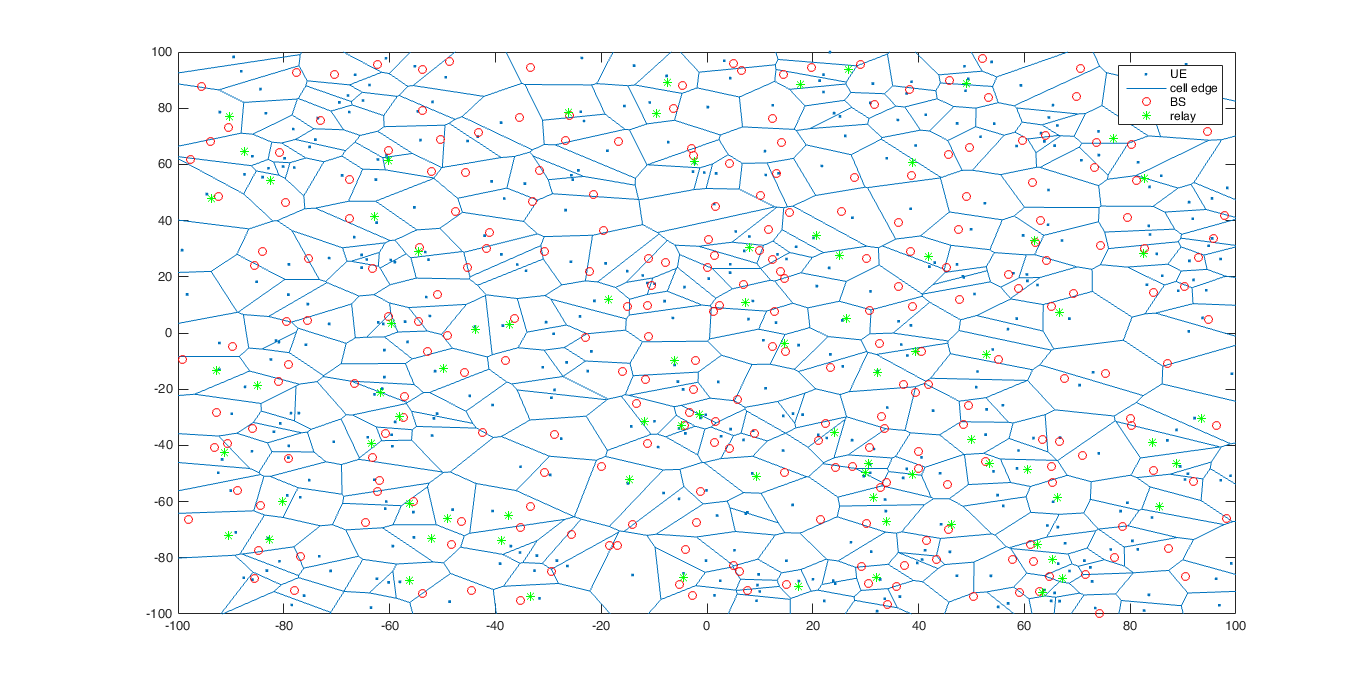
\includegraphics[height = 2.8in,width=4.5in,angle=00]{figures/netLayoutSim.png}
\centering
\vspace{-2mm}
\caption{Sample Network Layout}
\label{plot4}
\end{figure}
\end{frame}

\begin{frame}{Results}
In the reference paper, there was a mistake in the derivation of expression for cooperation probability($\rho_3$) of policy $E_3$. \\
$\mathcal{E}_2$ was used in place of $\mathcal{E}_3$

\begin{equation*}
\mathcal{E}_3 = \frac{\lambda_2 z^2}{2\pi(\lambda_1+\lambda_2z^2)}
\end{equation*}

\begin{equation*}
\mathcal{E}_2 = \frac{\lambda_2}{2\pi(\lambda_1+\lambda_2)}
\end{equation*}
\end{frame}

\begin{frame}{Results}
\begin{figure}[!h]
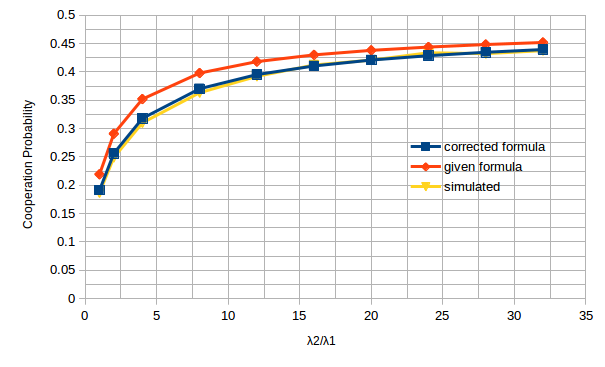
\includegraphics[width=10cm, height= 7cm]{figures/corrected.png}
\centering
\vspace{-2mm}
\caption{Cooperation probability of $E_3$.}
\label{plot1}
\end{figure}
\end{frame}


\begin{frame}{Results}
\begin{figure}[!h]
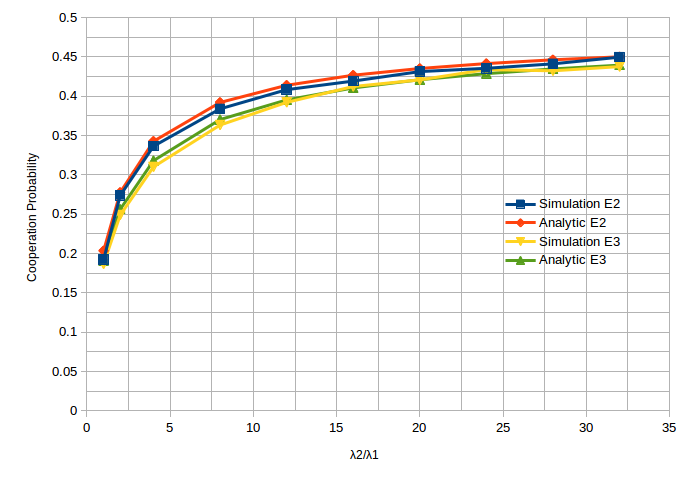
\includegraphics[width=10cm, height= 7cm]{figures/coopP.png}
\centering
\vspace{-2mm}
\caption{Cooperation probabilities v/s User ratio density. } 
\label{plot2}
\end{figure}
\end{frame}


\begin{frame}{Results}
\begin{figure}[!h]
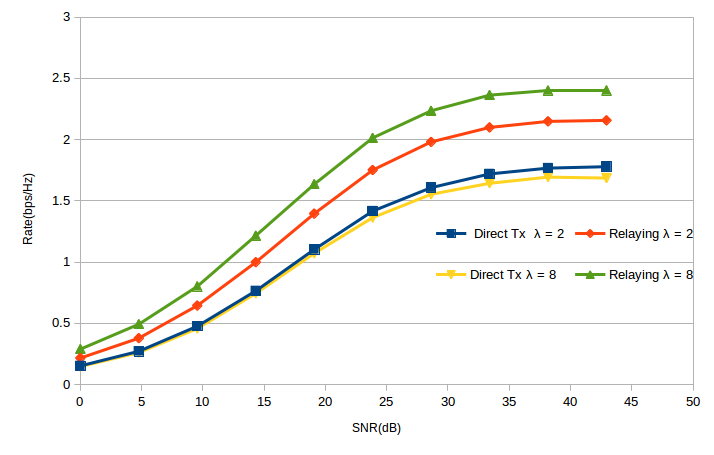
\includegraphics[width=\textwidth]{figures/rates.png}
\centering
\vspace{-2mm}
\caption{Per user average rate v/s SNR.}
\label{plot3}
\end{figure}
\end{frame}






% Placing a * after \section means it will not show in the



\begin{frame}{Future Work}{New Policy}
  \begin{itemize}
  \item
     In the policies $E_2$, $E_3$, only the first neighbour of the active UE is seen as a potential relay. 
    
   \item Any relay which is at a distance $r_2$ from active UE and satisfies $r_2<r_1, D < r_1$ can be treated as a potential relay
   \begin{figure}[!h]
        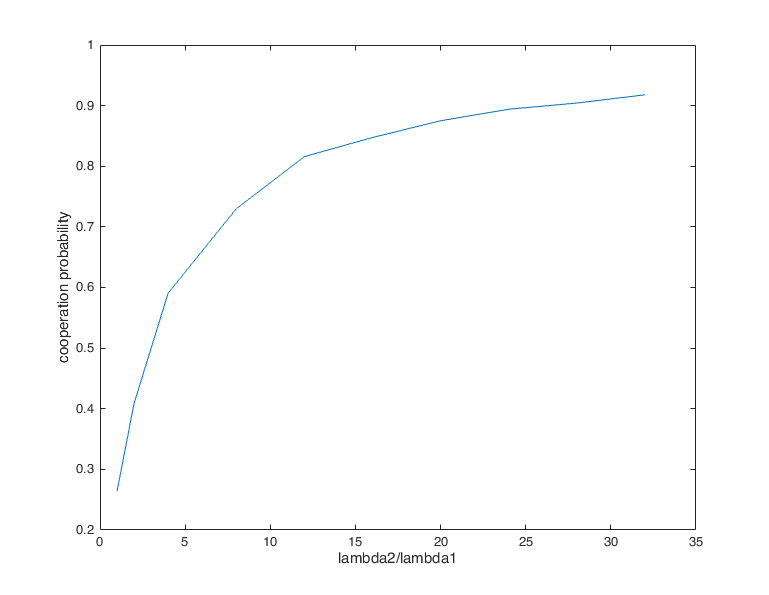
\includegraphics[width=7cm, height= 5cm]{figures/simulCoopE4.png}
        \centering
        \vspace{-2mm}
        \caption{Cooperation Probability v/s User density ratio}
        \label{plot3}
    \end{figure}    
 \end{itemize}   

\end{frame}

\begin{frame}{Future Work}{New Policy}
\vspace{1cm}
\begin{itemize}  
  \item
   This also means higher inteference
   \vspace{1cm}
  \item If rate decreases for some users, then there should be a way of deciding which users should use the relaying so that rate will be high for all users. 
  \end{itemize}
\end{frame}

\begin{frame}{Future Work}{$\beta_1$}
Power used by UE to transmit the common codeword in second phase $P_s^{m_1} = \beta_1 P_s^m$
\begin{itemize}  
  \item
   Currently, $\beta_1$ is obtained by optimizing the final rate
   \vspace{1cm}
   \pause
  \item This is not practical. 
  \pause
  \vspace{1cm}
  \item An algorithm can be developed to estimate $\beta_1$  
  \end{itemize}
\end{frame}

\begin{frame}{Future Work}{Power Control}
\vspace{1cm}
\begin{itemize}  
  \item
   We assumed that all nodes transmit at maximum power
   \vspace{1cm}
   \pause
  \item A distance based power control method can be applied 
  \end{itemize}
\end{frame}


\begin{frame}{}
\centering
\textbf{Thank You!!}


\end{frame}
\end{document}